\documentclass[aspectratio=169,11pt]{beamer}

% =============================================================================
% TEMPLATE - MACROECONOMIA II | LICENCIATURA EN ECONOMIA | CIDE
% Compilacion normal: pdflatex (o latexmk).
% Compilacion con bibliografía: pdflatex -> biber -> pdflatex -> pdflatex.
% =============================================================================

% --- Idioma, tipografia y matematicas -----------------------------------------
\usepackage[utf8]{inputenc}
\IfFileExists{spanish.ldf}{
  \usepackage[spanish,es-nodecimaldot]{babel}
}{
  \usepackage[english]{babel}
}
\usepackage{graphicx}
\usepackage{amsmath,amssymb}
\usepackage{array,tabularx}
\IfFileExists{booktabs.sty}{
  \usepackage{booktabs}
}{
  \providecommand{\toprule}{\hline}
  \providecommand{\midrule}{\hline}
  \providecommand{\bottomrule}{\hline}
}
\usepackage[table]{xcolor}

% --- Bibliografia opcional ----------------------------------------------------
% La bibliografia queda apagada para que el
% template base compile sin ejecutar Biber ni depender de biblatex.
% Cuando se agreguen referencias, 
% cambiar \usarBibliografiafalse por \usarBibliografiatrue
\newif\ifusarBibliografia
\usarBibliografiafalse

\ifusarBibliografia
  \IfFileExists{csquotes.sty}{\usepackage{csquotes}}{}
  \IfFileExists{apa.bbx}{
    \usepackage[backend=biber,style=apa,sorting=nyt]{biblatex}
  }{
    % Respaldo para instalaciones locales sin biblatex-apa.
    \usepackage[backend=biber,style=authoryear,sorting=nyt]{biblatex}
  }
  \IfFileExists{References.bib}{
    \addbibresource{References.bib}
  }{
    \addbibresource{References.bib.bib}
  }
\fi

% --- Paleta: azul marino, blanco y grises neutros ------------------
\definecolor{CIDENavy}{RGB}{3,25,54}
\definecolor{CIDEBlue}{RGB}{5,35,75}
\definecolor{CIDEInk}{RGB}{25,34,45}
\definecolor{CIDEGray}{RGB}{101,112,126}
\definecolor{CIDEGrayLight}{RGB}{243,244,246}


\setbeamercolor{normal text}{fg=CIDEInk,bg=white}
\setbeamercolor{structure}{fg=CIDEBlue}
\setbeamercolor{alerted text}{fg=CIDEBlue}
\setbeamercolor{title}{bg=CIDEBlue,fg=white}
\setbeamercolor{subtitle}{fg=CIDEInk}
\setbeamercolor{frametitle}{bg=CIDEBlue,fg=white}
\setbeamercolor{palette primary}{bg=CIDEBlue,fg=white}
\setbeamercolor{palette secondary}{bg=CIDEBlue,fg=white}
\setbeamercolor{palette tertiary}{bg=CIDENavy,fg=white}
\setbeamercolor{palette quaternary}{bg=CIDENavy,fg=white}
\setbeamercolor{section in head/foot}{bg=CIDENavy,fg=white}
\setbeamercolor{section in head/foot shaded}{bg=CIDENavy,fg=white!50}
\setbeamercolor{mini frame}{bg=white,fg=white}
\setbeamercolor{mini frame shaded}{bg=white!35,fg=white!35}
\setbeamercolor{upper separation line head}{bg=CIDENavy}
\setbeamercolor{lower separation line head}{bg=CIDEBlue}
\setbeamercolor{block title}{bg=CIDEBlue,fg=white}
\setbeamercolor{block body}{bg=CIDEGrayLight,fg=CIDEInk}
\setbeamercolor{block title alerted}{bg=CIDENavy,fg=white}
\setbeamercolor{block body alerted}{bg=CIDEGrayLight,fg=CIDEInk}
\setbeamercolor{caption name}{fg=CIDEBlue}
\setbeamercolor{section in toc}{fg=CIDEBlue}
\setbeamercolor{section in toc shaded}{fg=CIDEGray}

% --- Tipografia ---------------------------------------------------------------
\setbeamerfont{author in head/foot}{size=\tiny}
\setbeamerfont{institute in head/foot}{size=\tiny}
\setbeamerfont{title in head/foot}{size=\tiny}

% --- Geometria general --------------------------------------------------------
\setbeamersize{text margin left=0.70cm,text margin right=0.70cm}
\setlength{\leftmargini}{1.2em}
\setlength{\leftmarginii}{1.1em}
\setlength{\abovecaptionskip}{0.25em}
\setlength{\belowcaptionskip}{0pt}

% Navegacion superior con nombres de seccion y mini-indicadores consecutivos.
\useoutertheme[subsection=false]{miniframes}
\setbeamertemplate{navigation symbols}{}
\setbeamertemplate{mini frame}[circle]
\setbeamertemplate{mini frame in current subsection}[circle]

% Evita que Beamer distribuya las secciones a lo ancho de toda la pagina.
% Solo modifica el espaciado de la navegacion de miniframes.
\makeatletter
\patchcmd{\insertnavigation}
  {\hskip-1.875ex plus-1fill}
  {\hskip-1.875ex}
  {}{}
\patchcmd{\sectionentry}
  {\box\beamer@sectionbox\hskip1.875ex plus 1fill}
  {\box\beamer@sectionbox\hskip1.875ex}
  {}{}
\makeatother
\setbeamertemplate{caption}[numbered]
\setbeamertemplate{section in toc}[circle]
\setbeamertemplate{subsection in toc}[circle]
\setbeamertemplate{itemize item}{\raisebox{0.15ex}{\tiny$\blacktriangleright$}}
\setbeamertemplate{itemize subitem}{\raisebox{0.15ex}{\tiny$\bullet$}}
\setbeamertemplate{enumerate item}[circle]

% Banda de titulo de cada diapositiva.
\setbeamertemplate{frametitle}{%
  \nointerlineskip
  \begin{beamercolorbox}[
    wd=\paperwidth,
    ht=3.05ex,
    dp=1.05ex,
    leftskip=0.42cm,
    rightskip=0.42cm
  ]{frametitle}
    \usebeamerfont{frametitle}\insertframetitle
  \end{beamercolorbox}%
}

% Pie en dos niveles: autor/institucion y nombre corto/paginacion.
\setbeamertemplate{footline}{%
  \leavevmode
  \vbox{%
    \offinterlineskip
    \hbox{%
      \begin{beamercolorbox}[wd=.72\paperwidth,ht=2.05ex,dp=.55ex,leftskip=.35cm]{palette secondary}
        \usebeamerfont{author in head/foot}\insertshortauthor
      \end{beamercolorbox}%
      \begin{beamercolorbox}[wd=.28\paperwidth,ht=2.05ex,dp=.55ex,rightskip=.35cm plus1fil]{palette secondary}
        \hfill\usebeamerfont{institute in head/foot}\insertshortinstitute
      \end{beamercolorbox}%
    }%
    \hbox{%
      \begin{beamercolorbox}[wd=.86\paperwidth,ht=1.85ex,dp=.50ex,leftskip=.35cm]{palette tertiary}
        \usebeamerfont{title in head/foot}\insertshorttitle
      \end{beamercolorbox}%
      \begin{beamercolorbox}[wd=.14\paperwidth,ht=1.85ex,dp=.50ex,center]{palette tertiary}
        \usebeamerfont{title in head/foot}\insertframenumber{} / \inserttotalframenumber
      \end{beamercolorbox}%
    }%
    \hbox to \paperwidth{%
      \hfill
      \raisebox{0.68cm}[0pt][0pt]{%
        \includegraphics[height=0.58cm,keepaspectratio]{\RutaLogoCIDE}%
      }%
      \hspace{0.18cm}%
    }%
  }%
  \vskip0pt
}

% Logo CIDE automatico en la esquina inferior derecha de todas las diapositivas.
\newcommand{\RutaLogoCIDE}{Figuras/General/logocide.png}

% Portada
\setbeamertemplate{title page}{%
  \vspace*{0.35cm}
  \centering
  \begin{beamercolorbox}[wd=\textwidth,sep=0.24cm,center,rounded=false]{title}
    \usebeamerfont{title}\inserttitle\par
  \end{beamercolorbox}
  \vspace{0.25cm}
  {\usebeamerfont{subtitle}\usebeamercolor[fg]{subtitle}\insertsubtitle\par}
  \vfill
  {\usebeamerfont{author}\insertauthor\par}
  \vspace{0.35cm}
  {\usebeamerfont{institute}\insertinstitute\par}
  \vfill
  {\usebeamerfont{date}\insertdate\par}
  \vspace{0.25cm}
}

% --- Comandos reutilizables ---------------------------------------------------
% Cambiar esta ruta una vez por cada presentacion/sesion.
\newcommand{\FigurasSesion}{Figuras/01_Introducción}

% Uso: \figura[0.65\textheight]{nombre-del-archivo.png}
\newcommand{\figura}[2][0.65\textheight]{%
  \includegraphics[width=\linewidth,height=#1,keepaspectratio]{\FigurasSesion/#2}%
}

% Uso: \cidehighlight{concepto clave}
\newcommand{\cidehighlight}[1]{\textcolor{CIDEBlue}{\bfseries #1}}

% Hipervínculos
\hypersetup{
  colorlinks=true,
  urlcolor=blue,
  linkcolor=.,
  citecolor=.,
  filecolor=.
}

% Filas alternadas para tablas: escribe \rowcolors{2}{CIDEGrayLight}{white}
\newcolumntype{Y}{>{\raggedright\arraybackslash}X}

% Diapositiva de contenido al comenzar cada seccion.
% Cambia \sectiontocfalse si prefieres no generarlas automaticamente.
\newif\ifsectiontoc
\sectiontocfalse
\AtBeginSection[]{%
  \ifsectiontoc
    \begin{frame}{Contenido}
      \tableofcontents[currentsection,hideothersubsections]
    \end{frame}
  \fi
}

% =============================================================================
% METADATOS DE CADA PRESENTACION
% =============================================================================
\title[Macroeconomía II]{Sesión 1 \\ Introducción al curso}
\subtitle{Macroeconomía II}
\author[LECO]{Arturo López}
\institute[CIDE]{Centro de Investigación y Docencia Económicas (CIDE)}
\date[Otoño 2026]{Licenciatura en Economía, Otoño 2026}
% =============================================================================
\begin{document}
% =============================================================================

\begin{frame}
  \titlepage
\end{frame}

% \begin{frame}{Contenido}
%    \tableofcontents
% \end{frame}

\section{Información general}

\begin{frame}[t]{Curso: Macroeconomía II}
  \vspace{0.6cm}

  \textbf{Profesor:} Arturo López Pérez\\
  \href{mailto:alopezperez.2605@gmail.com}{alopezperez.2605@gmail.com}

  \vspace{0.4cm}

  \textbf{Laboratorista:} Jibran Elias Mejia\\
  \href{mailto:jibran.elias@alumnos.cide.edu}{jibran.elias@alumnos.cide.edu}

  \vspace{0.4cm}

  \textbf{Horario:} Martes y jueves, de 8:00 a 9:30 hrs.

  \vspace{0.4cm}

  \textbf{Aula:} TBC

  \vspace{0.4cm}

  \textbf{Página del curso:} \href{}{GitHub} (en construcción)
\end{frame}

\section{Su profesor}

\begin{frame}{¿Quién soy?}
  \begin{itemize}
    \item Economista y Maestro en Economía por el CIDE.
    \item Experiencia laboral: investigación económica (INEGI, Dirección General de Integración, Análisis e Investigación), analista (Nielsen, Área de Data Science) y analista financiero (Renovo Home Partners, FP\&A Department).

    \item Actualmente: Subdirector de Modelos Matemáticos en la Dirección General de Análisis Macroeconómico de la Secretaría de Hacienda y Crédito Público (SHCP)... y su profesor de Macro II.

    \item Mis intereses de investigación incluyen economía monetaria, macroeconomía internacional, macroeconomía computacional y econometría.
  \end{itemize}
\end{frame}

\begin{frame}{Investigación}
  Algunos documentos de trabajo (títulos tentativos):

  \begin{itemize}
    \item López, Arturo y Chávez, Emmanuel (2026).
    \textit{Labor Market Effects of Minimum Wage Increases and Fiscal Stimulus: Evidence from Mexico's Northern Border}.

    \item López, Arturo y Villicaña, Emiliano (2026).
    \textit{The Anatomy of Household Inflation in Mexico}.
    Documento de trabajo en revisión.

    \item Solís, Pavel y López, Arturo (2026).
    \textit{How Exogenous Are Monetary Policy Surprises in Mexico?}.
  \end{itemize}
\end{frame}

\section{Presentación del curso}

\begin{frame}{Presentación del curso}
  \begin{itemize}
    \item Curso de macroeconomía \textit{moderna}
    \item El enfoque se basa en modelos \cidehighlight{dinámicos} de \cidehighlight{equilibrio general} con \cidehighlight{fundamentos microeconómicos}:
    \begin{itemize}
      \item Agentes representativos que toman decisiones óptimas, sujetos a sus preferencias, tecnología y restricciones...
      \item ... en equilibrio general (precios y cantidades se ajustan de forma endógena para que la oferta sea igual a la demanda en todos los mercados involucrados).
    \end{itemize}
    \item En este curso: 
    \begin{itemize}
      \item Estudio de las causas y mecanismos de propagación de las fluctuaciones macroeconómicas de \cidehighlight{corto plazo}, así como el papel de la política macroeconómica de estabilización.
    \end{itemize}
  \end{itemize}
\end{frame}


\begin{frame}{Objetivos y prerrequisitos}

\small

\begin{itemize}
  \setlength{\itemsep}{0.65em}

  \item \textbf{Objetivos:}
  \begin{itemize}
    \setlength{\itemsep}{0.25em}

    \item Desarrollar las herramientas conceptuales y analíticas necesarias
    para construir, resolver e interpretar modelos macroeconómicos con
    fundamentos microeconómicos.

    \item Identificar y comprender los supuestos y mecanismos que sustentan
    los principales resultados teóricos.

    \item Interpretar datos macroeconómicos y evidencia empírica a la luz de
    los modelos estudiados en clase.
  \end{itemize}

  \item \textbf{Prerrequisitos:}
  \begin{itemize}

    \item Optimización estática con restricciones y conceptos fundamentales de microeconomía.

  \end{itemize}
\end{itemize}

\end{frame}



\begin{frame}{Evaluación}
  \begin{itemize}
    \item Examen parcial: \textbf{30\%}.
    \item Examen final: \textbf{50\%}.
    \item Laboratorio: \textbf{20\%}.
  \end{itemize}
\end{frame}


\begin{frame}[t]{Libros de texto}

\footnotesize

\begin{columns}[T,onlytextwidth]
  \begin{column}{0.56\textwidth}
    \textbf{Textos principales}

    \vspace{0.08cm}
    \hrule
    \vspace{0.12cm}

    \begin{itemize}
      \setlength{\itemsep}{0.35em}

      \item \textbf{WS:} Williamson, Stephen D. (2018).
      \textit{Macroeconomics}, 6th ed. Pearson Education Limited.

      \item \textbf{KP:} Kurlat, Pablo (2020).
      \textit{A Course in Modern Macroeconomics}.
      Apuntes de clase, Stanford University.

      \item \textbf{SUW:} Schmitt-Grohé, S., Uribe, M. y Woodford, M. (2022).
      \textit{International Macroeconomics: A Modern Approach}.
      Princeton University Press.
    \end{itemize}
  \end{column}

  \begin{column}{0.40\textwidth}
    \textbf{Uso dentro del curso}

    \vspace{0.08cm}
    \hrule
    \vspace{0.12cm}

    \begin{itemize}
      \setlength{\itemsep}{0.45em}

      \item \textbf{Parte I: economía cerrada.}
      Se seguirá principalmente la exposición de \textbf{WS}, mientras que \textbf{KP} se utilizará para profundizar en los aspectos más técnicos de los modelos.

      \item \textbf{Parte II: economía abierta.}
      Se seguirá principalmente la exposición de \textbf{SUW}.
    \end{itemize}
  \end{column}

\end{columns}

\vspace{0.18cm}
\hrule
\vspace{0.12cm}

\textbf{Evidencia y aplicaciones.}
Cada tema se complementará con evidencia empírica y aplicaciones de la literatura académica. Los artículos de investigación permitirán evaluar las predicciones de los modelos analizados en clase.

\end{frame}


\begin{frame}[t]{Calendario y temas del curso}

\vspace{0.10cm}

\begin{center}
\begingroup
\fontsize{6.5}{7.2}\selectfont
\renewcommand{\arraystretch}{1.06}
\setlength{\tabcolsep}{0.07cm}
\setlength{\arrayrulewidth}{0.35pt}

\begin{tabular}{|c|c|l|}
\hline
\parbox[c]{1.15cm}{\centering\bfseries Semana} &
\parbox[c]{2.45cm}{\centering\bfseries Sesiones} &
\parbox[c]{9.70cm}{\raggedright\bfseries Tema} \\
\hline

\textbf{1} &
25 y 27 ago. &
\parbox[c]{9.70cm}{\raggedright Introducción al curso. Conducta del consumidor y de la empresa (I).} \\
\hline

\textbf{2} &
1 y 3 sep. &
\parbox[c]{9.70cm}{\raggedright Conducta del consumidor y de la empresa (II). Equilibrio general.} \\
\hline

\textbf{3} &
8 y 10 sep. &
\parbox[c]{9.70cm}{\raggedright Elección intertemporal de consumo y ahorro.} \\
\hline

\textbf{4} &
15 y 17 sep. &
\parbox[c]{9.70cm}{\raggedright Inversión y acumulación de capital. Equilibrio general dinámico.} \\
\hline

\textbf{5} &
22 y 24 sep. &
\parbox[c]{9.70cm}{\raggedright Modelo de ciclos reales de negocios.} \\
\hline

\textbf{6} &
29 sep. y 1 oct. &
\parbox[c]{9.70cm}{\raggedright Modelo nuevo keynesiano.} \\
\hline

\textbf{7} &
6 y 8 oct. &
\parbox[c]{9.70cm}{\raggedright\textbf{Repaso y primer examen parcial.}} \\
\hline

\textbf{8} &
13 y 15 oct. &
\parbox[c]{9.70cm}{\raggedright Desempleo.} \\
\hline

\textbf{9} &
20 y 22 oct. &
\parbox[c]{9.70cm}{\raggedright Determinantes de la cuenta corriente (I).} \\
\hline

\textbf{10} &
27 y 29 oct. &
\parbox[c]{9.70cm}{\raggedright Determinantes de la cuenta corriente (II).} \\
\hline

\textbf{11} &
3 y 5 nov. &
\parbox[c]{9.70cm}{\raggedright Términos de intercambio, tasa de interés mundial, tarifas y cuenta corriente (I).} \\
\hline

\textbf{12} &
10 y 12 nov. &
\parbox[c]{9.70cm}{\raggedright Términos de intercambio, tasa de interés mundial, tarifas y cuenta corriente (II).} \\
\hline

\textbf{13} &
17 y 19 nov. &
\parbox[c]{9.70cm}{\raggedright Determinantes del tipo de cambio real.} \\
\hline

\textbf{14} &
24 y 26 nov. &
\parbox[c]{9.70cm}{\raggedright Rigidez nominal, política monetaria y desempleo (I).} \\
\hline

\textbf{15} &
1 y 3 dic. &
\parbox[c]{9.70cm}{\raggedright Rigidez nominal, política monetaria y desempleo (II).} \\
\hline

&
7--18 dic. &
\parbox[c]{9.70cm}{\raggedright\textbf{Examen final} (fecha por determinar).} \\
\hline

\end{tabular}
\endgroup
\end{center}

\vspace{0.06cm}

{\fontsize{6.1}{6.8}\selectfont
\textit{Nota: La distribución de temas entre evaluaciones puede cambiar dependiendo del avance del curso.}
}
\end{frame}



\section{Ideas generales sobre el curso}

\begin{frame}{¿Qué busca la teoría macroeconómica?}
  ¿Para qué sirven los modelos (macro)económicos?
  \begin{itemize}
    \item Describir, explicar y predecir el \cidehighlight{comovimiento de variables agregadas} a lo largo del ciclo económico: producción, empleo, inflación, consumo, inversión y balanza comercial, etc.
    \item Identificar los \cidehighlight{choques} que originan las fluctuaciones macroeconómicas y los \cidehighlight{mecanismos} mediante los cuales sus efectos se propagan en el tiempo.
    \item Construir \cidehighlight{experimentos contrafactuales} para evaluar los posibles efectos de distintas políticas económicas.
    \item En la vida real, los modelos nos ayudan a interpretar la coyuntura, elaborar pronósticos y formular recomendaciones de política macroeconómica.
  \end{itemize}
\end{frame}


\begin{frame}[t]{La (macro)economía confronta modelos con evidencia}

\footnotesize

\begin{columns}[T,onlytextwidth]

  % ── Modelo ──────────────────────────────────────────────────────────────────
  \begin{column}{0.45\textwidth}

    \textbf{La teoría organiza la pregunta}

    \begin{itemize}
      \setlength{\itemsep}{0.35em}

      \item Los modelos aíslan mecanismos y hacen explícitos los supuestos
      detrás de una explicación económica.

      \item Ejemplo de un modelo: una empresa elige su demanda de trabajo para maximizar beneficios:
      \vspace{-0.15cm}
      \[
      \max_{n\geq 0}\left\{f(n)-wn\right\},
      \]
    \vspace{-0.15cm}
    donde \(n\) es el empleo, \(f(n)\) la producción y \(w\) el salario real.
    \end{itemize}

  \end{column}

  % ── Evidencia ───────────────────────────────────────────────────────────────
  \begin{column}{0.52\textwidth}

    {\footnotesize \bfseries Tasa de desocupación en México}\\[-0.02cm]
    {\scriptsize \% de la Población Económicamente Activa}\\[-0.02cm]

    \vspace{0.08cm}

    \centering
    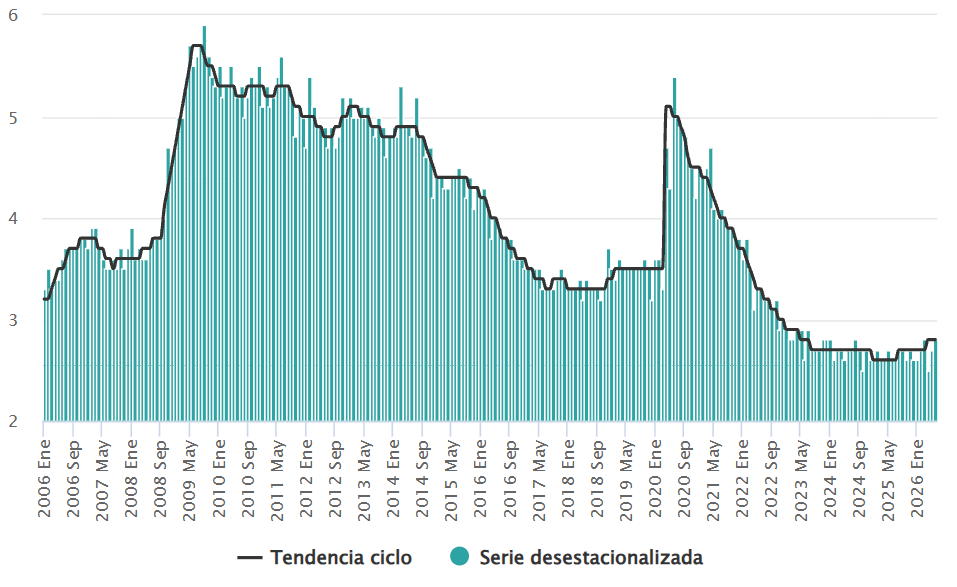
\includegraphics[
      width=\linewidth,
      height=4.45cm,
      keepaspectratio
    ]{Figuras/01_Introducción/Tasa de desocupación.png}

    \vspace{0.02cm}

    \raggedright
    {\tiny
    \textit{Fuente:} INEGI, Banco de Información Económica (BIE).
    }

  \end{column}

\end{columns}

\end{frame}


\begin{frame}[t]{Ahora, lo mismo para un conjunto de series macroeconómicas}

\footnotesize

\begin{columns}[T,onlytextwidth]

  % ── Modelo de equilibrio general ────────────────────────────────────────────
  \begin{column}{0.46\textwidth}

    El objetivo ya no es explicar una sola variable, sino el
    \textbf{comovimiento} de series macroeconómicas

    \vspace{0.12cm}

    \textbf{Ej. modelo de equilibrio general}

    \vspace{0.08cm}

    \textbf{Hogares:}
    \vspace{-0.2cm}
    \[
      \max_{\{c_t,n_t,k_{t+1}\}}
      \sum_{t=0}^{\infty}
      \beta^t
      \bigl[u(c_t)-v(n_t)\bigr]
    \]

    \vspace{-0.40cm}

    \[
    \text{s.t. } \ 
      c_t+k_{t+1}
      =
      w_tn_t+(r_t+1-\delta)k_t .
    \]

    \vspace{-0.05cm}

    \textbf{Empresas:}
    \vspace{-0.2cm}
    \[
      \max_{\{k_t,n_t\}}
      \left\{
      f(k_t,n_t)
      -r_tk_t-w_tn_t
      \right\}.
    \]

    \vspace{-0.05cm}

    \textbf{Equilibrio de mercados:}
    \vspace{-0.2cm}
    \[
      y_t=c_t+i_t,
      \qquad
      k_{t+1}=(1-\delta)k_t+i_t.
    \]

    \vspace{0.06cm}

    %Un mismo conjunto de choques debe explicar simultáneamente la dinámica
    %observada en todas las series.

  \end{column}

  % ── Series macroeconómicas ─────────────────────────────────────────────────
  \begin{column}{0.56\textwidth}
    
    \centering

    {\bfseries Un sistema de variables macroeconómicas}\\[-0.02cm]
    {\scriptsize México y Estados Unidos, 2004--2026}

    \vspace{0.08cm}

    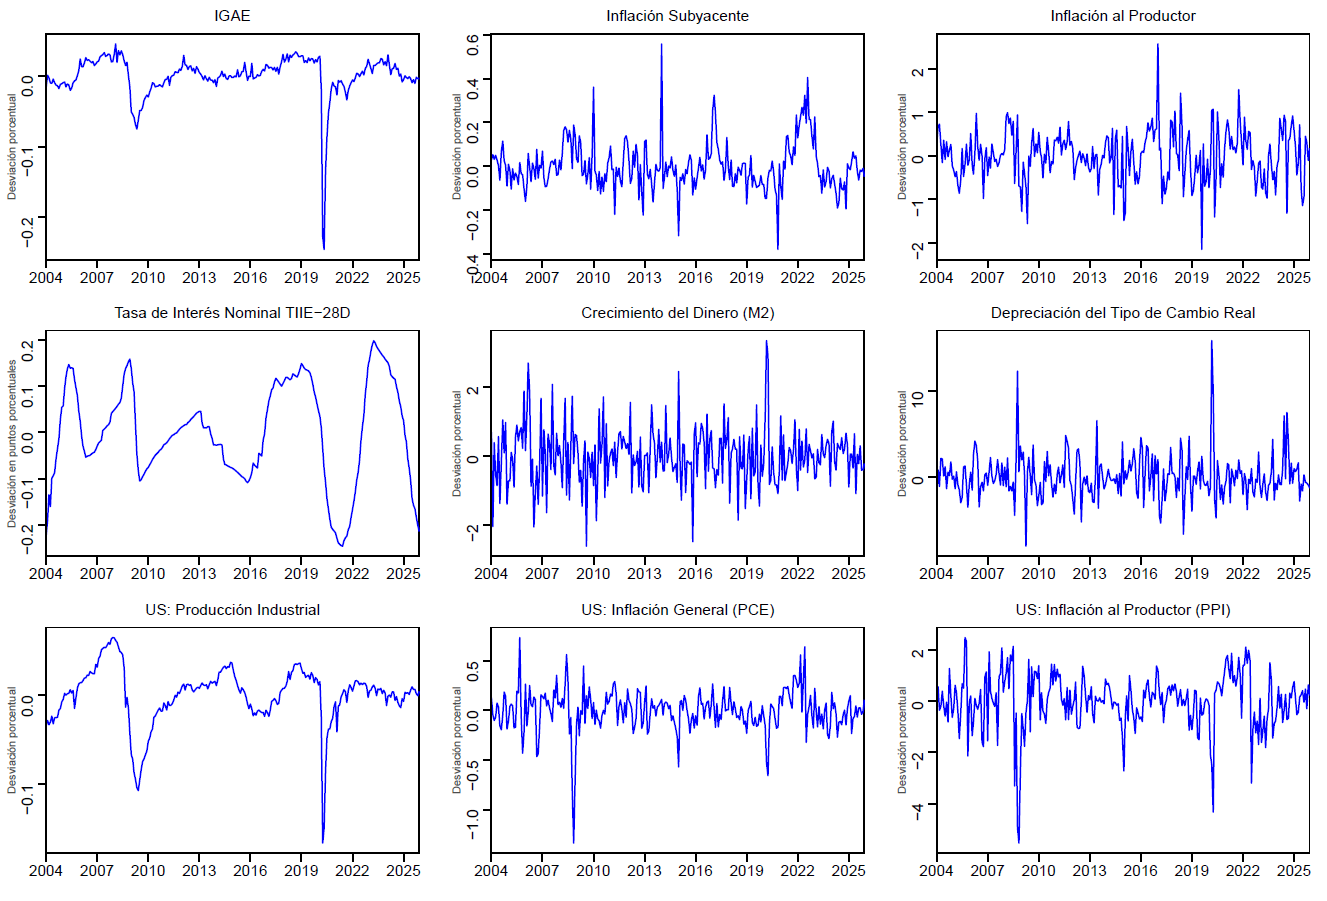
\includegraphics[
      width=\linewidth,
      height=5cm,
      keepaspectratio
    ]{Figuras/01_Introducción/Series Macro.png}

    \vspace{0.01cm}

    \raggedright
    {\tiny
    \textit{Fuente:} Elaboración propia con datos de INEGI, Banco de México y FRED.
    }

  \end{column}

\end{columns}

\end{frame}

\begin{frame}
  La macroeconomía necesita de la interacción entre modelos y datos.

    \textbf{Los datos disciplinan el modelo}
    \begin{itemize}

      \item La evidencia permite identificar patrones, evaluar predicciones
      y detectar mecanismos que los modelos deben ser capaces de explicar.
    \end{itemize}

    \textbf{Datos sin teoría: volar a ciegas}
    \begin{itemize}
      \item Dejar que los datos ``hablen por sí solos'' puede conducir a interpretaciones engañosas o carentes de contenido económico.
      \item Todo trabajo empírico tiene un modelo económico detrás (aunque sea implícito)
      \item Muchas preguntas de política económica son contrafactuales: para responderlas se requiere un modelo que permita comparar escenarios alternativos.
    \end{itemize}
\end{frame}

\begin{frame}{Modelos macroeconómicos en la práctica}

  Los modelos que estudiaremos durante el curso son versiones pequeñas y
  simplificadas de los que se emplean en la literatura académica y en
  bancos centrales. Sin embargo, conservan los mecanismos económicos
  esenciales.

  \vspace{0.3cm}

  \textbf{Ejemplos de modelos utilizados por bancos centrales:}

  \begin{itemize}
    \setlength{\itemsep}{0.45em}

    \item \href{https://www.newyorkfed.org/research/policy/dsge}
    {\textbf{FRBNY DSGE Model}}:
    modelo de la Fed de Nueva York.

    \item \href{https://www.ecb.europa.eu/pub/pdf/scpwps/ecbwp944.pdf}
    {\textbf{New Area-Wide Model (NAWM)}}:
    modelo para la zona del euro del Banco Central Europeo.

    \item \href{https://www.federalreserve.gov/econres/edo-models-about.htm}
    {\textbf{Estimated Dynamic Optimization (EDO) Model}}:
    modelo de la Junta de Gobernadores de la Fed.
  \end{itemize}

\end{frame}




\begin{frame}{Hacia un modelo macroeconómico}

  \small

  \begin{itemize}
    \setlength{\itemsep}{0.35em}

    \item En la próxima sesión: el primer modelo macroeconómico moderno.

    \item El modelo será extremadamente sencillo:
    \begin{itemize}
      \setlength{\itemsep}{0.15em}
      \item un consumidor ``representativo'';
      \item una empresa ``representativa'';
      \item un solo periodo;
      \item un único bien;
      \item un único factor de producción: el trabajo;
      \item ninguna fricción o imperfección de mercado;
      \item una \alert{\textbf{``economía de Robinson Crusoe''}} con dos agentes representativos.
    \end{itemize}

    \item Aun así, incorporará dos características fundamentales de la
    macroeconomía moderna:
    \begin{enumerate}
      \setlength{\itemsep}{0.1em}
      \item fundamentos microeconómicos;
      \item equilibrio general.
    \end{enumerate}

    \item En el resto del curso construiremos modelos progresivamente más
    complejos y realistas.

  \end{itemize}

\end{frame}
%
% REFERENCIAS (activa \usarBibliografiatrue y descomenta este frame)
% \begin{frame}[allowframebreaks]{Referencias}
%   \printbibliography[heading=none]
% \end{frame}

\end{document}
